\documentclass[12pt, a4paper]{report}

% --- UNIVERSAL PREAMBLE BLOCK ---
\usepackage[
  margin=2cm
]{geometry}
\usepackage{fontspec}

\usepackage[turkish, bidi=basic, provide=*]{babel}

\babelprovide[import, onchar=ids fonts]{turkish}
\babelprovide[import, onchar=ids fonts]{english}

\usepackage{enumitem}
\setlist[itemize]{label=-}

\usepackage{dirtree}
\usepackage{listings}
\usepackage{xcolor}
\usepackage{booktabs}
\usepackage{parskip}
\usepackage{graphicx}
\graphicspath{{images/}}
\usepackage{tikz}
\usetikzlibrary{positioning, shapes.multipart, arrows.meta}

%----------BOX----------

\usepackage{tcolorbox}

\newtcolorbox{block}[1]{
  colback=blue!5!white,
  colframe=blue!75!black,
  fonttitle=\bfseries,
  title=#1,
  arc=1mm,
  sharp corners=south
}

%----------METADATA----------
\usepackage{titling}
\usepackage{titlesec}
\titleformat{\chapter}[block]{\Large\bfseries}{\thechapter.}{0.5em}{}

\newcommand{\projectname}{Proje 3: Veritabanı Güvenliği ve Erişim Kontrolü}
\newcommand{\studentnumber}{22290121}

\title{BLM4522 - Ağ Tabanlı Paralel Dağıtım Sistemleri Vize Projesi}
\author{Melike Vurucu}
\date{\today}

%----------TITLE LAYOUT----------
\pretitle{
\begin{center}\LARGE}
  \posttitle{\\[0.5em]\large\projectname
\end{center}}
\preauthor{
\begin{center}}
  \postauthor{\ (\studentnumber)
\end{center}}

%----------CODE STYLE----------
\definecolor{codegray}{rgb}{0.95,0.95,0.95}
\definecolor{codeblue}{rgb}{0.0,0.3,0.6}
\definecolor{codegreen}{rgb}{0.1,0.5,0.1}
\definecolor{codepurple}{rgb}{0.4,0.0,0.5}
\definecolor{codered}{rgb}{0.7,0.0,0.0}

\lstdefinestyle{sqlstyle}{
  backgroundcolor=\color{codegray},
  commentstyle=\color{codegreen}\itshape,
  keywordstyle=\color{codeblue}\bfseries,
  stringstyle=\color{codered},
  basicstyle=\ttfamily\small,
  breaklines=true,
  captionpos=b,
  keepspaces=true,
  showspaces=false,
  showstringspaces=false,
  tabsize=4,
  frame=single,
  framerule=0.5pt,
  language=SQL,
  extendedchars=true,
  literate=
  {İ}{İ}1 {ı}{ı}1
  {Ş}{Ş}1 {ş}{ş}1
  {Ğ}{Ğ}1 {ğ}{ğ}1
  {Ü}{Ü}1 {ü}{ü}1
  {Ö}{Ö}1 {ö}{ö}1
  {Ç}{Ç}1 {ç}{ç}1
  {â}{â}1 {Â}{Â}1,
  morekeywords={
    ROLE, LOGIN, PASSWORD, CREATEDB, CREATEROLE,
    CONNECTION, LIMIT, SECURITY, DEFINER, ENABLE,
    FORCE, ROW, LEVEL, POLICY, USING, WITH, CHECK,
    TRIGGER, AFTER, EACH, EXECUTE, FUNCTION, RETURNS,
    LANGUAGE, plpgsql, DECLARE, BEGIN, END, RETURN,
    QUERY, RAISE, NOTICE, EXCEPTION, WHEN, THEN,
    ELSIF, TG_OP, TG_TABLE_NAME, NEW, OLD, JSONB,
    to_jsonb, current_user, current_setting, gen_salt,
    crypt, pgp_sym_encrypt, pgp_sym_decrypt, encode, decode
  }
}

\lstset{style=sqlstyle}

% hyperref must be loaded last
\usepackage{hyperref}
\hypersetup{
  colorlinks=true,
  linkcolor=black!60!black,
  urlcolor=blue!60!black,
  citecolor=blue!60!black
}

%----------DOCUMENT----------
\begin{document}

\maketitle
\tableofcontents

\chapter{Giriş}

Bu projede PostgreSQL üzerinde veritabanı güvenliğinin temel bileşenleri uygulamalı olarak gösterilmiştir.

Bu proje kapsamında \textbf{Doğa Pazarlama} adlı kurgusal bir pazarlama firmasının veritabanı oluşturulup bu veritabanı üzerinde aşağıdaki güvenlik katmanları oluşturulmuş ve eyleme geçirilmiştir:

\begin{enumerate}
  \item \textbf{Erişim Yönetimi}: PostgreSQL rolleri, \texttt{scram-sha-256} şifreli kimlik doğrulama, \texttt{GRANT}/\texttt{REVOKE} ve Satır Seviyesinde Güvenlik (RLS).
  \item \textbf{Veri Şifreleme}: \texttt{pgcrypto} eklentisi ile sütun seviyesinde PGP simetrik şifreleme.
  \item \textbf{SQL Injection Testleri}: Güvensiz ve güvenli giriş fonksiyonlarının karşılaştırmalı demosu.
  \item \textbf{Denetim Günlükleri}: Tetikleyici tabanlı otomatik denetim kaydı ve şüpheli aktivite tespiti.
\end{enumerate}

\section{Veritabanı Şeması}

\textbf{doga\_pazarlama} veritabanı beş uygulama tablosu ile bir denetim günlüğü tablosundan oluşmaktadır. Şekil~\ref{fig:er} tablo ilişkilerini ve hassas alanları göstermektedir. \textcolor{red!70!black}{\textbf{Kırmızı}} ile işaretlenmiş alanlar şifreli veya hash'lenmiş hassas veri içermektedir.

\tikzset{
  ent/.style={
    rectangle split, rectangle split parts=2,
    draw=blue!60!black, very thick,
    rectangle split part fill={blue!15!white, white},
    font=\small\ttfamily,
    align=left,
    inner sep=5pt,
    text width=3.6cm
  }
}

\begin{figure}[h!]
  \centering
  \resizebox{\linewidth}{!}{%
    \begin{tikzpicture}[
        fk/.style={->, >=Stealth, dashed, thick, blue!50!black, line width=1.2pt}
      ]

      \node[ent] (emp) at (0,0) {
        \normalfont\bfseries\small\sffamily employees
        \nodepart{second}
        \underline{employee\_id}\ \ PK\\[1pt]
        first\_name, last\_name\\[1pt]
        email\ UNIQUE\\[1pt]
        department, job\_title\\[1pt]
        hire\_date\\[1pt]
        \textcolor{red!70!black}{\bfseries salary}\ \textcolor{red!70!black}{\small[PGP]}
      };

      \node[ent] (cust) at (6,0) {
        \normalfont\bfseries\small\sffamily customers
        \nodepart{second}
        \underline{customer\_id}\ \ PK\\[1pt]
        first\_name, last\_name\\[1pt]
        email\ UNIQUE, city\\[1pt]
        \textcolor{red!70!black}{\bfseries credit\_card}\ \textcolor{red!70!black}{\small[PGP]}\\[1pt]
        \textcolor{red!70!black}{\bfseries national\_id}\ \textcolor{red!70!black}{\small[PGP]}
      };

      \node[ent] (ua) at (12,0) {
        \normalfont\bfseries\small\sffamily user\_accounts
        \nodepart{second}
        \underline{account\_id}\ \ PK\\[1pt]
        username\ UNIQUE\\[1pt]
        email\ UNIQUE\\[1pt]
        \textcolor{red!70!black}{\bfseries password\_hash}\ \textcolor{red!70!black}{\small[bcrypt]}\\[1pt]
        role
      };

      \node[ent] (trx) at (0,-6.5) {
        \normalfont\bfseries\small\sffamily transactions
        \nodepart{second}
        \underline{transaction\_id}\ \ PK\\[1pt]
        customer\_id\ FK\\[1pt]
        amount, type\\[1pt]
        description, created\_at
      };

      \node[ent] (la) at (6,-6.5) {
        \normalfont\bfseries\small\sffamily login\_attempts
        \nodepart{second}
        \underline{attempt\_id}\ \ PK\\[1pt]
        username, ip\_address\\[1pt]
        success, attempted\_at
      };

      \node[ent] (al) at (12,-6.5) {
        \normalfont\bfseries\small\sffamily audit\_log
        \nodepart{second}
        \underline{log\_id}\ \ PK\\[1pt]
        table\_name, operation\\[1pt]
        old\_data\ JSONB\\[1pt]
        new\_data\ JSONB\\[1pt]
        changed\_by, changed\_at
      };

      % FK: transactions.customer_id -> customers (N:1)
      \draw[fk] (trx.north east) -- ++(0.5,0)
      |- node[near start, right, font=\footnotesize\sffamily, xshift=3pt] {N:1}
      (cust.south);

      % Legend
      \node[draw=gray!60, fill=yellow!8, rounded corners=3pt,
      align=left, font=\footnotesize\sffamily, inner sep=7pt] at (6,-9.5) {
        \textcolor{red!70!black}{\textbf{[PGP]}}\ \ pgcrypto PGP simetrik şifreleme ile korunan alan\quad
        \textcolor{red!70!black}{\textbf{[bcrypt]}}\ \ bcrypt hash ile korunan alan
      };

    \end{tikzpicture}%
  }
  \caption{doga\_pazarlama ER diyagramı}
  \label{fig:er}
\end{figure}

\begin{figure}[h!]
  \centering
  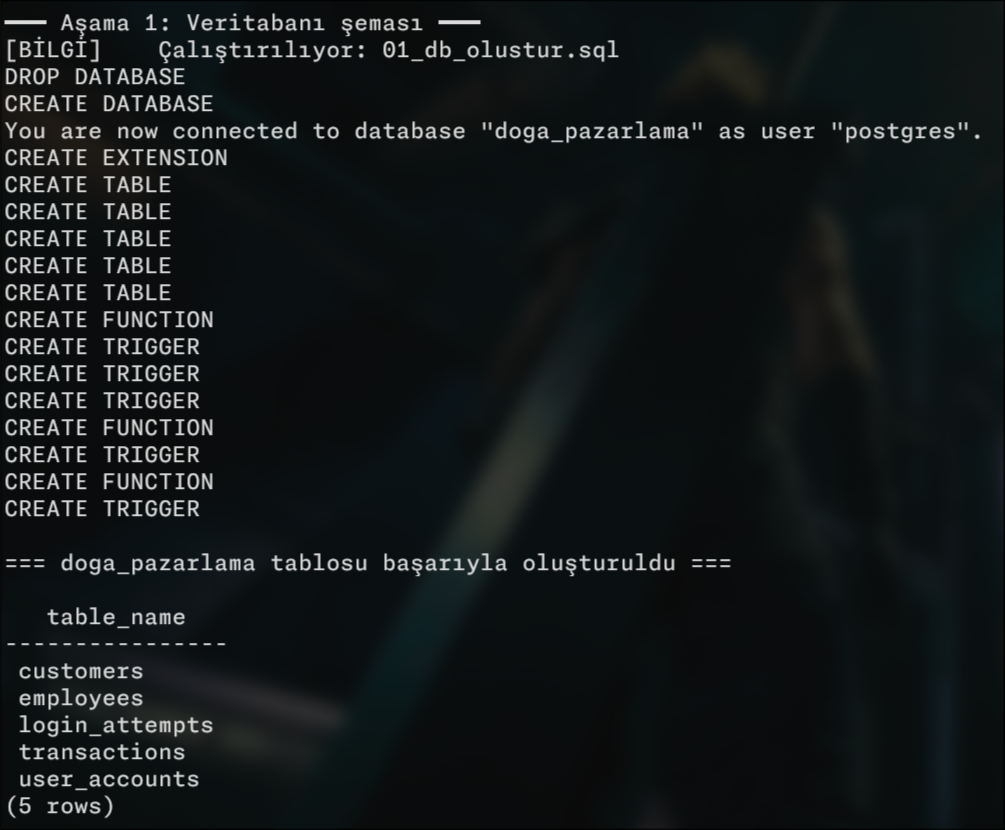
\includegraphics[width=\linewidth]{2_create_table}
  \caption{Veritabanı ve tabloların oluşturulması (01\_db\_olustur.sql)}
  \label{fig:create-table}
\end{figure}

\begin{figure}[h!]
  \centering
  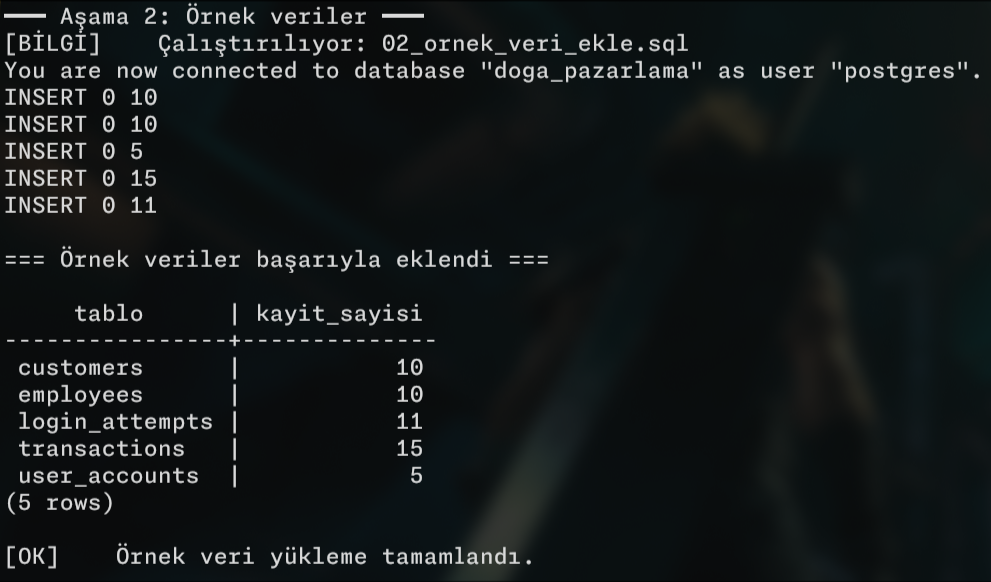
\includegraphics[width=\linewidth]{3_insert_data}
  \caption{Örnek verilerin yüklenmesi (02\_ornek\_veri\_ekle.sql)}
  \label{fig:insert-data}
\end{figure}

Doğa Pazarlama adlı hayali şirkete ait veritabanının oluşturulma nedeni ise gerçek hayatta özellikle de şirketlerde erişim kontrolü ve şifreleme gibi güvenlik önlemlerinin hayati bir önem taşımasıdır.

\section{Şema Tetikleyicileri}

Veritabanı şeması (\texttt{01\_db\_olustur.sql}) üç yardımcı tetikleyici içermektedir:

\begin{itemize}
  \item \textbf{normalize\_email}: \texttt{employees}, \texttt{customers} ve \texttt{user\_accounts} tablolarında \texttt{INSERT}/\texttt{UPDATE} sırasında e-posta adresini küçük harfe çevirir ve baştaki/sondaki boşlukları siler.
  \item \textbf{set\_hire\_date}: \texttt{employees} tablosuna \texttt{INSERT} sırasında \texttt{hire\_date} sağlanmamışsa günün tarihini atar.
  \item \textbf{validate\_transaction\_amount}: \texttt{transactions} tablosuna sıfır veya negatif tutar girilmesini engeller.
\end{itemize}

\chapter{Kullanılan Teknolojiler}

\begin{itemize}
  \item \textbf{PostgreSQL 18}: Açık kaynaklı, nesne-ilişkisel veritabanı yönetim sistemi.
  \item \textbf{pgcrypto}: PostgreSQL eklentisi; simetrik/asimetrik şifreleme ve hash fonksiyonları sağlar. \texttt{pgp\_sym\_encrypt}, \texttt{crypt}, \texttt{gen\_salt} fonksiyonları kullanılmıştır.
  \item \textbf{PL/pgSQL}: PostgreSQL'in prosedürel SQL dili; trigger fonksiyonları ve güvenli giriş fonksiyonları bu dilde yazılmıştır.
  \item \textbf{Bash}: Kurulum scriptlerinin orkestrasyon katmanı.
  \item \textbf{scram-sha-256}: RFC 7677 tabanlı kimlik doğrulama protokolü; PostgreSQL 14'ten itibaren varsayılan olarak etkin.
\end{itemize}

\section{Proje Klasör Yapısı}

Aşağıda projenin klasör yapısı verilmiştir:

\vspace{1em}
\dirtree{%
  .1 proje3-guvenlik/.
  .2 config/.
  .3 pg\_hba\_example.conf \qquad \textit{\# Kimlik doğrulama yapılandırması}.
  .2 scripts/.
  .3 00\_run\_all.sh \qquad \textit{\# Toplu çalıştırma scripti}.
  .3 01\_db\_olustur.sql \qquad \textit{\# Veritabanı şeması ve tetikleyiciler}.
  .3 02\_ornek\_veri\_ekle.sql \qquad \textit{\# Örnek veriler}.
  .3 03\_rol\_ekle.sql \qquad \textit{\# Roller ve kimlik doğrulama}.
  .3 04\_access\_control.sql \qquad \textit{\# Yetkilendirme ve RLS}.
  .3 05\_sifreleme.sql \qquad \textit{\# Sütun şifreleme}.
  .3 06\_sql\_injection.sql \qquad \textit{\# SQL injection demo}.
  .3 07\_audit\_log.sql \qquad \textit{\# Denetim tetikleyicileri}.
  .3 08\_demo.sql \qquad \textit{\# Kapsamlı demo}.
  .2 proje3-rapor.pdf.
}

\newpage
\chapter{Erişim Yönetimi}

\section{Şifreli Kimlik Doğrulama}

PostgreSQL, istemci kimlik doğrulamasını \texttt{pg\_hba.conf} dosyası üzerinden yönetir. Bu projede \textbf{scram-sha-256} yöntemi tercih edilmiştir.

\texttt{scram-sha-256} protokolünün \texttt{md5}'e göre avantajları:
\begin{itemize}
  \item Şifre ağ üzerinden düz metin veya zayıf hash olarak iletilmez.
  \item Replay (tekrar oynatma) saldırılarına karşı koruma sağlar.
  \item RFC 7677 standardını uygular; modern ve güvenilir bir protokoldür.
  \item PostgreSQL 14+ sürümlerinde \texttt{password\_encryption} varsayılanı \texttt{scram-sha-256} olarak değiştirilmiştir.
\end{itemize}

\begin{lstlisting}[caption={pg\_hba.conf — scram-sha-256 yapılandırması}]
-- postgresql.conf
password_encryption = scram-sha-256

-- pg_hba.conf
local  doga_pazarlama  hr_manager      scram-sha-256
host   doga_pazarlama  hr_manager  127.0.0.1/32  scram-sha-256
\end{lstlisting}

\begin{figure}[h!]
  \centering
  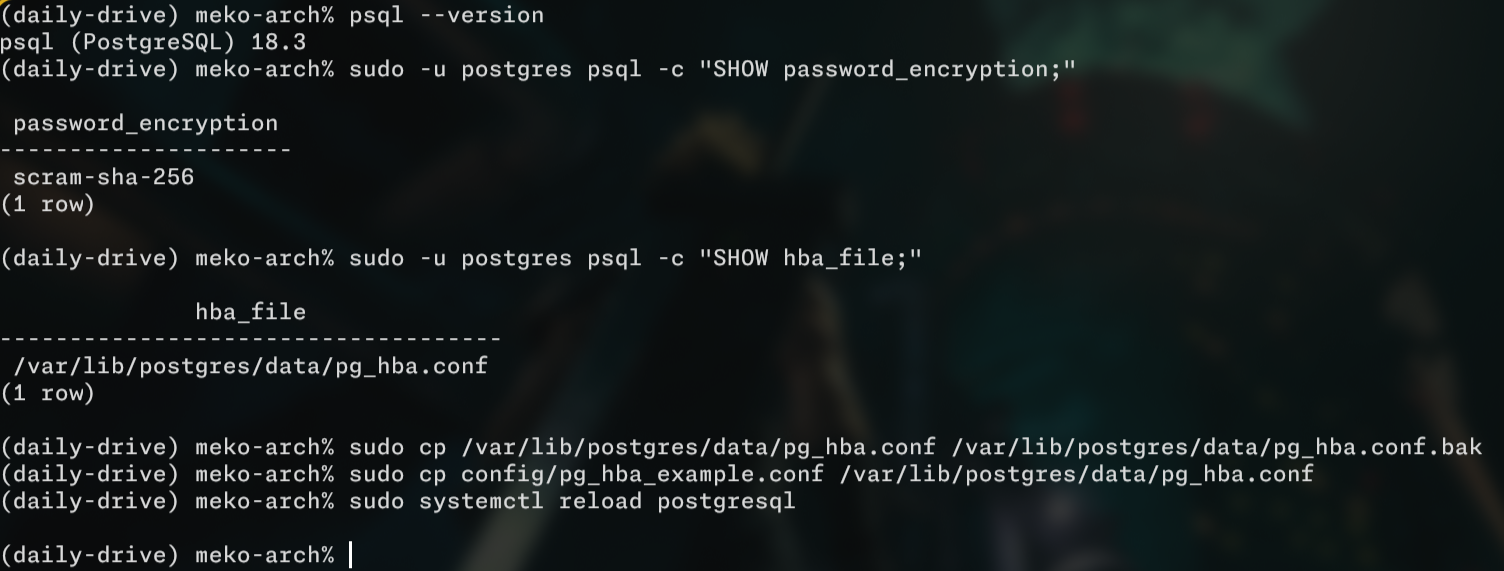
\includegraphics[width=\linewidth]{1_pg_hba_config}
  \caption{pg\_hba.conf yapılandırması ve scram-sha-256 doğrulaması}
  \label{fig:pg-hba}
\end{figure}

\section{PostgreSQL Rolleri}

Prensip: \textbf{en az ayrıcalık (principle of least privilege)}. Her rol yalnızca iş işlevinin gerektirdiği tablolara ve işlemlere erişebilir.

\begin{table}[h]
  \centering
  \begin{tabular}{@{}lll@{}}
    \toprule
    \textbf{Rol} & \textbf{Şifre} & \textbf{Erişim} \\
    \midrule
    \texttt{doga\_admin}      & \texttt{DogaAdmin@21!Password.} & Veritabanı yönetimi \\
    \texttt{hr\_manager}      & \texttt{HR@Manager\#2021!}      & employees: tam CRUD \\
    \texttt{finance\_analyst} & \texttt{F1n@nce\#2024!}         & transactions: CRUD, customers: SELECT \\
    \texttt{customer\_service}& \texttt{CustServ\#2024!}        & customers: CRUD, transactions: SELECT \\
    \texttt{readonly\_user}   & \texttt{R3@dOnly\#2024!}        & Tüm tablolar: yalnızca SELECT \\
    \texttt{app\_service}     & \texttt{AppS3rv1ce\#2024!}      & user\_accounts: SELECT, login\_attempts: INSERT \\
    \bottomrule
  \end{tabular}
  \caption{PostgreSQL rolleri ve erişim düzeyleri}
\end{table}

\begin{lstlisting}[caption={Rol oluşturma örneği (03\_rol\_ekle.sql)}]
CREATE ROLE hr_manager WITH
    LOGIN
    PASSWORD 'HR@Manager#2021!'
    CONNECTION LIMIT 5;
\end{lstlisting}

\begin{figure}[h!]
  \centering
  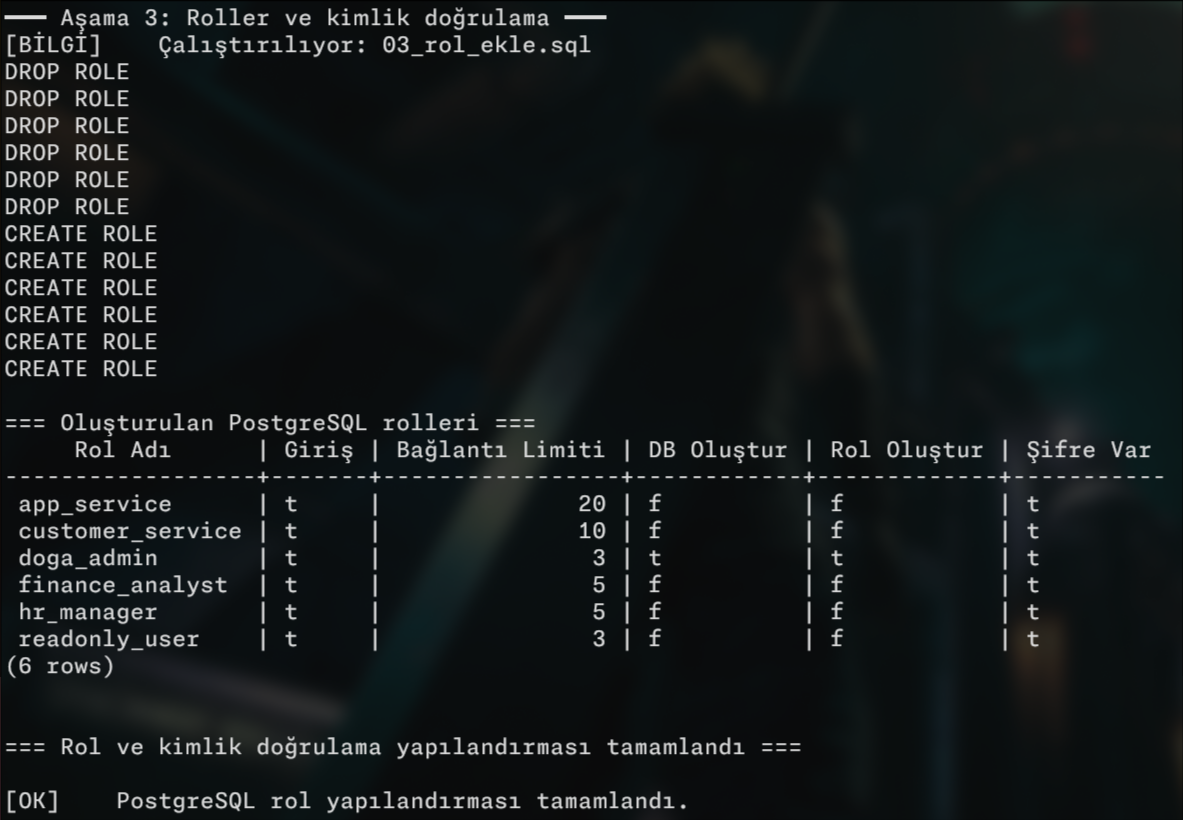
\includegraphics[width=\linewidth]{4_create_role}
  \caption{PostgreSQL rollerinin oluşturulması (03\_rol\_ekle.sql)}
  \label{fig:create-role}
\end{figure}

\section{GRANT / REVOKE}

\texttt{PUBLIC} rolünün varsayılan şema erişimi kaldırılmış; her role yalnızca ihtiyaç duyduğu tablo ve dizi erişimleri verilmiştir:

\begin{lstlisting}[caption={Yetkilendirme örneği (04\_access\_control.sql)}]
-- Varsayilan PUBLIC erisimini kapat
REVOKE ALL ON SCHEMA public FROM PUBLIC;
REVOKE ALL ON ALL TABLES IN SCHEMA public FROM PUBLIC;

-- hr_manager: calisan yonetimi
GRANT SELECT, INSERT, UPDATE, DELETE ON employees TO hr_manager;
GRANT USAGE, SELECT ON SEQUENCE employees_employee_id_seq TO hr_manager;

-- finance_analyst: finansal raporlama
GRANT SELECT, INSERT, UPDATE ON transactions TO finance_analyst;
GRANT SELECT                  ON customers    TO finance_analyst;
GRANT USAGE, SELECT ON SEQUENCE transactions_transaction_id_seq TO finance_analyst;

-- app_service: yalnizca giris dogrulama ve log yazma
GRANT SELECT ON user_accounts  TO app_service;
GRANT INSERT ON login_attempts TO app_service;
GRANT USAGE, SELECT ON SEQUENCE login_attempts_attempt_id_seq TO app_service;
\end{lstlisting}

\section{Satır Seviyesinde Güvenlik (Row Level Security)}

RLS, aynı tablo üzerinde farklı kullanıcıların yalnızca izin verilen satırları görmesini sağlar. \texttt{employees} tablosuna üç politika uygulanmıştır:

\begin{lstlisting}[caption={RLS politikaları (04\_access\_control.sql)}]
ALTER TABLE employees ENABLE ROW LEVEL SECURITY;
ALTER TABLE employees FORCE ROW LEVEL SECURITY;

-- hr_manager tum calisanlari gorebilir
CREATE POLICY hr_full_access ON employees
    FOR ALL TO hr_manager
    USING (TRUE) WITH CHECK (TRUE);

-- doga_admin tum calisanlari gorebilir
CREATE POLICY admin_full_access ON employees
    FOR ALL TO doga_admin
    USING (TRUE) WITH CHECK (TRUE);

-- readonly_user yalnizca kendi departmanini gorebilir
-- (oturum acilirken: SET app.current_department = 'Finans')
CREATE POLICY dept_filtered_access ON employees
    FOR SELECT TO readonly_user
    USING (department = current_setting('app.current_department', TRUE));
\end{lstlisting}

\texttt{FORCE ROW LEVEL SECURITY} sayesinde tablo sahibi bile (superuser hariç) politikalara tabi tutulur.

\begin{figure}[h!]
  \centering
  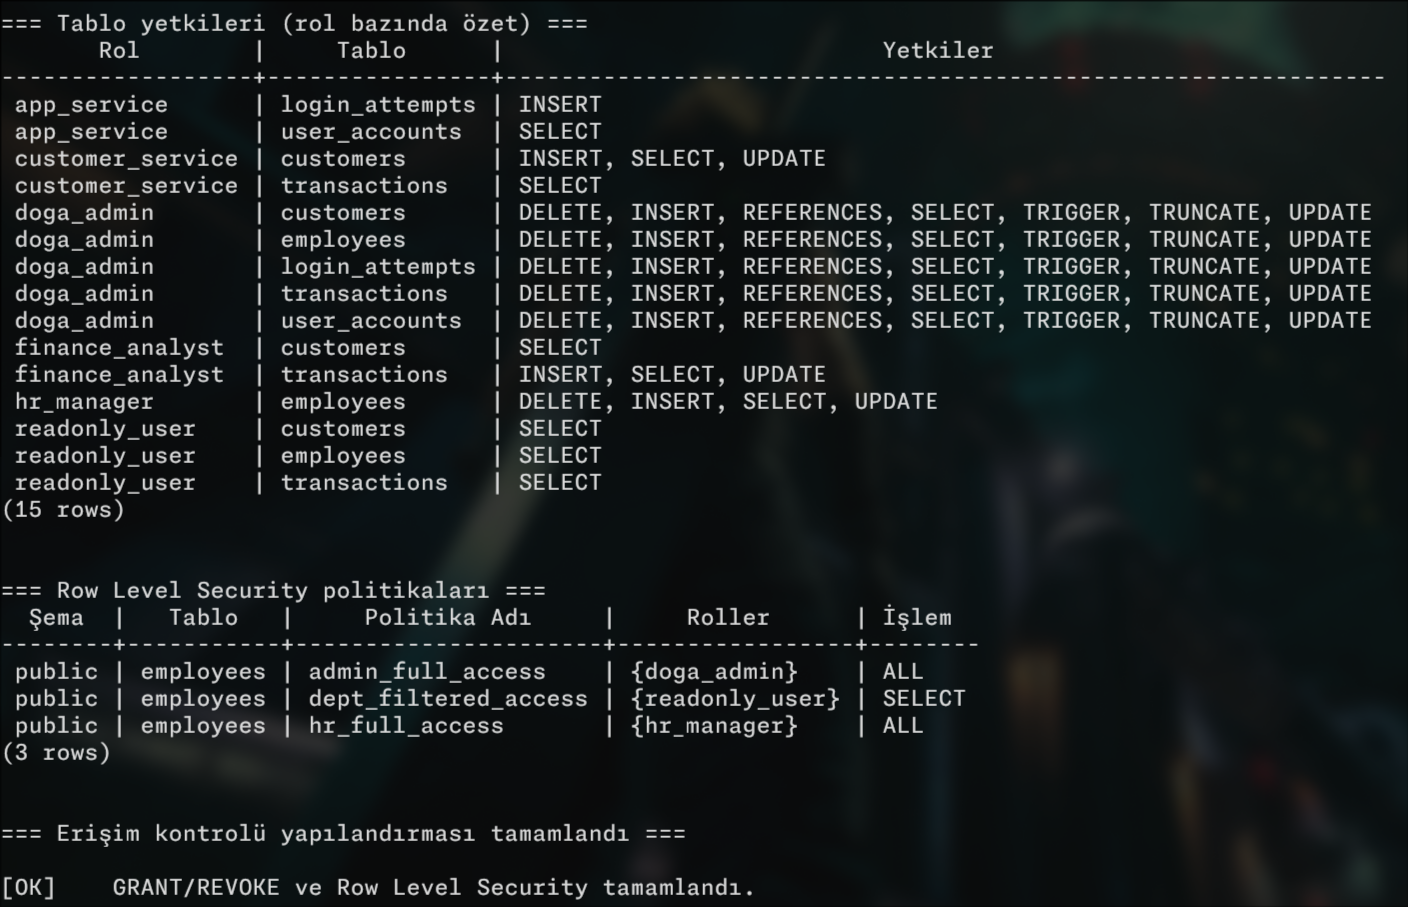
\includegraphics[width=\linewidth]{5_access_control}
  \caption{Tablo yetkileri ve RLS politikaları (04\_access\_control.sql)}
  \label{fig:access-control}
\end{figure}

\begin{figure}[h!]
  \centering
  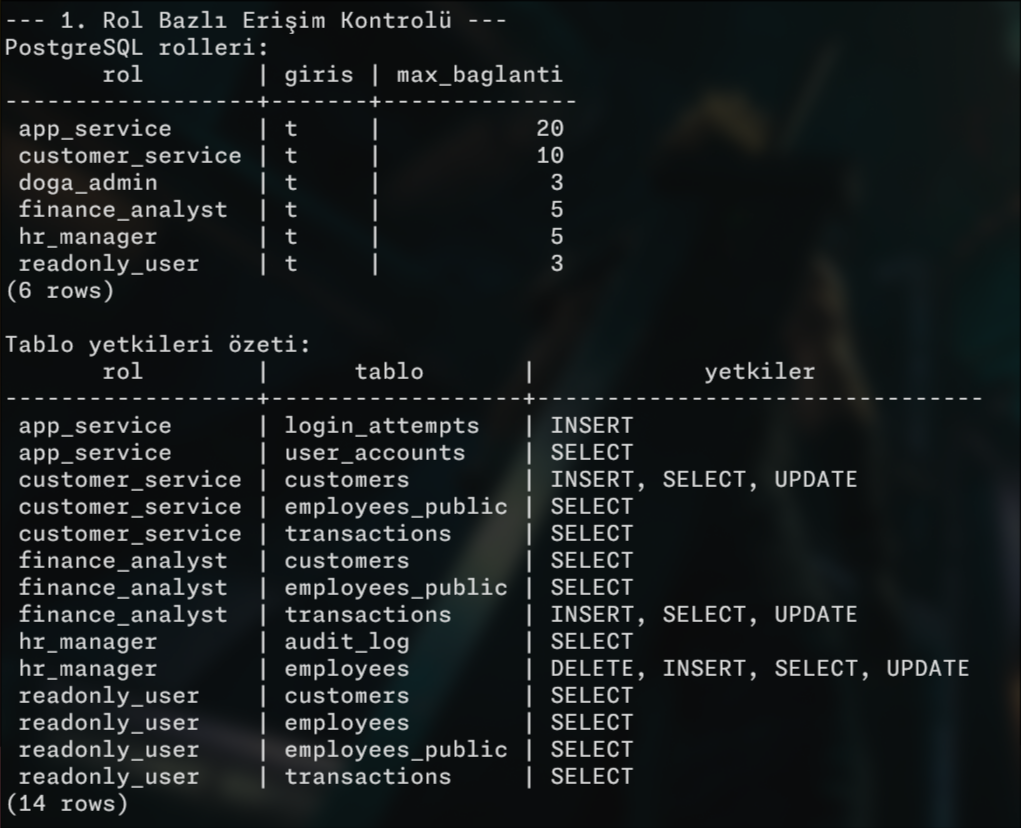
\includegraphics[width=\linewidth]{9_overview_roles}
  \caption{Rol bazlı erişim kontrolü — genel bakış (08\_demo.sql)}
  \label{fig:overview-roles}
\end{figure}

\chapter{Veri Şifreleme}

\section{pgcrypto ile Sütun Şifreleme}

PostgreSQL'in \texttt{pgcrypto} eklentisi, veri tabanı seviyesinde kriptografik işlemler gerçekleştirmeye olanak tanır. Bu projede \textbf{PGP simetrik şifreleme} (AES-256 tabanlı) kullanılmıştır.

Şifrelenen hassas alanlar:
\begin{itemize}
  \item \texttt{employees.salary} — çalışan maaş bilgisi
  \item \texttt{customers.credit\_card} — müşteri kredi kartı numarası
  \item \texttt{customers.national\_id} — TC kimlik numarası
\end{itemize}

\section{Yardımcı Fonksiyonlar}

İki \texttt{SECURITY DEFINER} fonksiyonu tanımlanmıştır:

\begin{lstlisting}[caption={Şifreleme ve çözme fonksiyonları (05\_sifreleme.sql)}]
-- Duz metni sifreler ve base64 TEXT olarak dondurur.
CREATE OR REPLACE FUNCTION encrypt_field(plain_text TEXT)
RETURNS TEXT LANGUAGE plpgsql SECURITY DEFINER AS $$
BEGIN
    IF plain_text IS NULL THEN RETURN NULL; END IF;
    RETURN encode(
        pgp_sym_encrypt(plain_text, current_setting('app.encryption_key')),
        'base64'
    );
END; $$;

-- Sifreli alani cozer; yalnizca yetkili roller cagirabilir.
CREATE OR REPLACE FUNCTION decrypt_field(encrypted_text TEXT)
RETURNS TEXT LANGUAGE plpgsql SECURITY DEFINER AS $$
BEGIN
    IF encrypted_text IS NULL THEN RETURN NULL; END IF;
    RETURN pgp_sym_decrypt(
        decode(encrypted_text, 'base64'),
        current_setting('app.encryption_key')
    );
END; $$;

-- Sifre cozme yetkisi yalnizca ihtiyac duyan rollere verilir.
REVOKE ALL ON FUNCTION decrypt_field(TEXT) FROM PUBLIC;
GRANT EXECUTE ON FUNCTION decrypt_field(TEXT)
    TO doga_admin, hr_manager, finance_analyst;
GRANT EXECUTE ON FUNCTION encrypt_field(TEXT) TO PUBLIC;
\end{lstlisting}

\begin{figure}[h!]
  \centering
  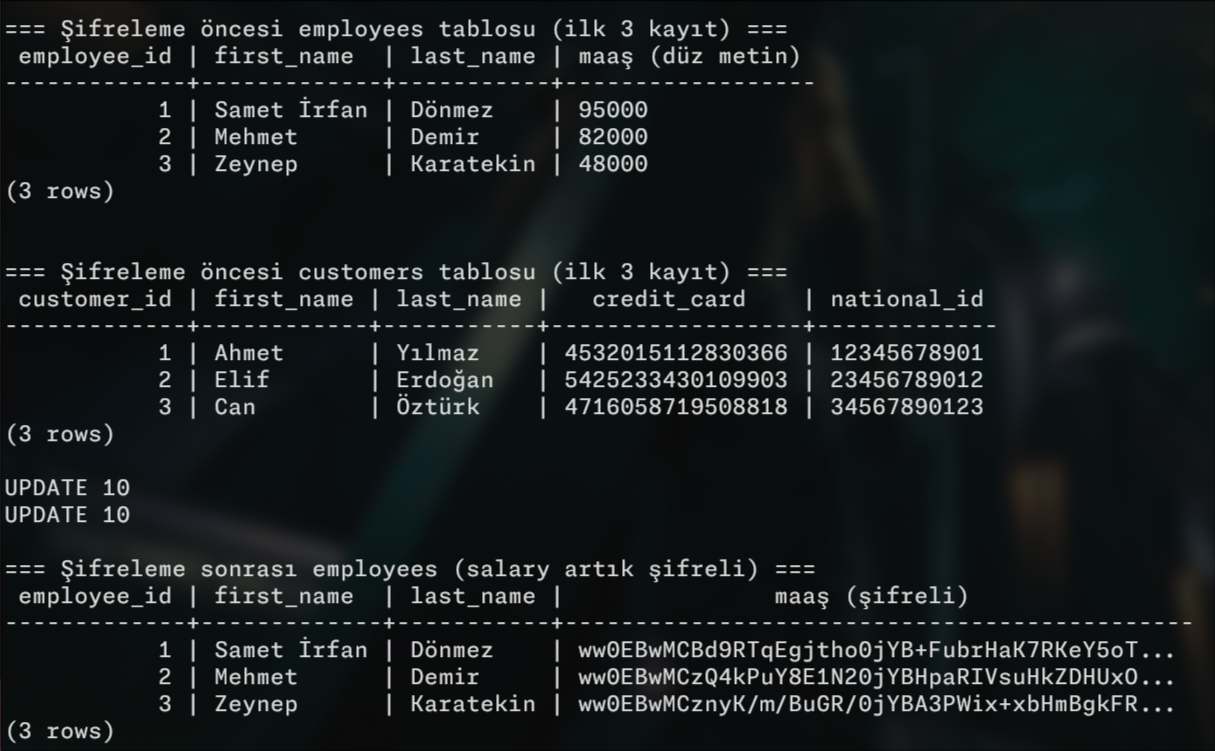
\includegraphics[width=\linewidth]{6_1_encryption}
  \caption{Şifreleme öncesi ve sonrası veri görünümü}
  \label{fig:enc-before-after}
\end{figure}

\section{Şifreleme Akışı}

Şifreleme anahtarı her veritabanı oturumunda uygulama tarafından ayarlanır:

\begin{lstlisting}[caption={Oturum bazlı şifreleme anahtarı}]
-- Her baglantida uygulama tarafindan bir deger atanmalidir.
SET app.encryption_key = 'uretimde-guclu-bir-anahtar-kullanin';

-- Veri ekleme
INSERT INTO employees (..., salary) VALUES (..., encrypt_field('95000'));

-- Yetkili okuma
SELECT decrypt_field(salary) FROM employees WHERE employee_id = 1;

-- Yetkisiz okuma (donen veri okunamaz)
SELECT salary FROM employees WHERE employee_id = 1;
-- Cikti: "wX4B..." (base64 kodlu sifreli veri)
\end{lstlisting}

\begin{figure}[h!]
  \centering
  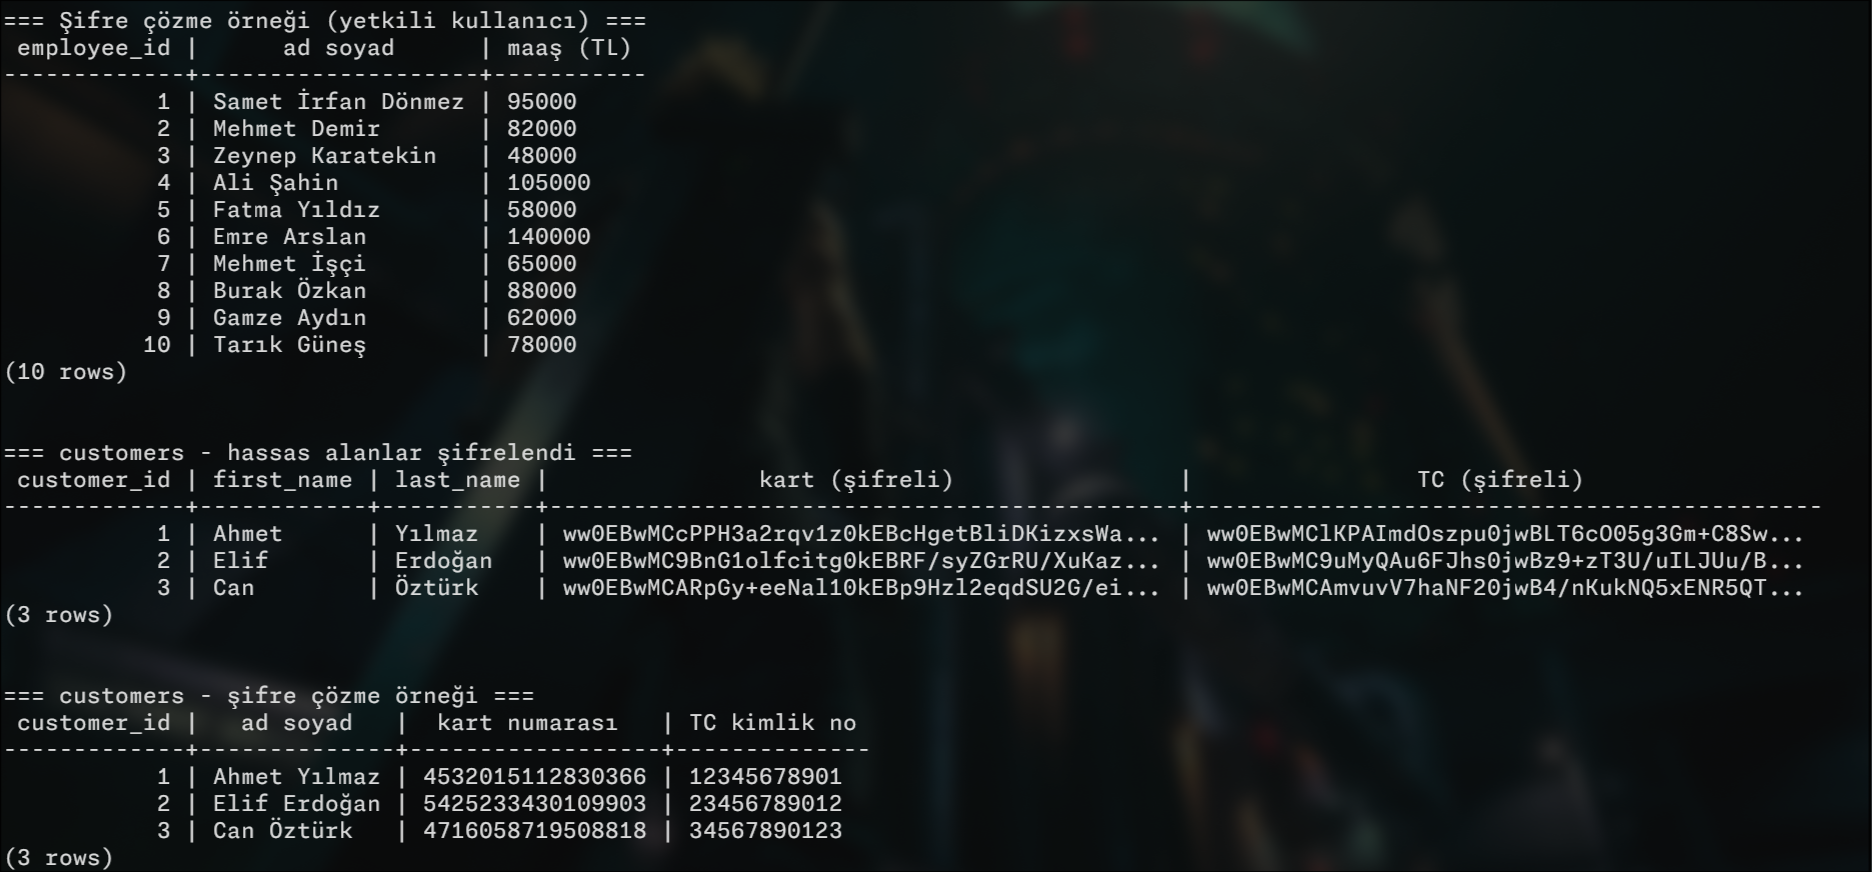
\includegraphics[width=\linewidth]{6_2_encryption}
  \caption{Şifre çözme örneği — yetkili kullanıcı maaş ve müşteri verilerini görüntülüyor}
  \label{fig:enc-decrypt}
\end{figure}

\begin{figure}[h!]
  \centering
  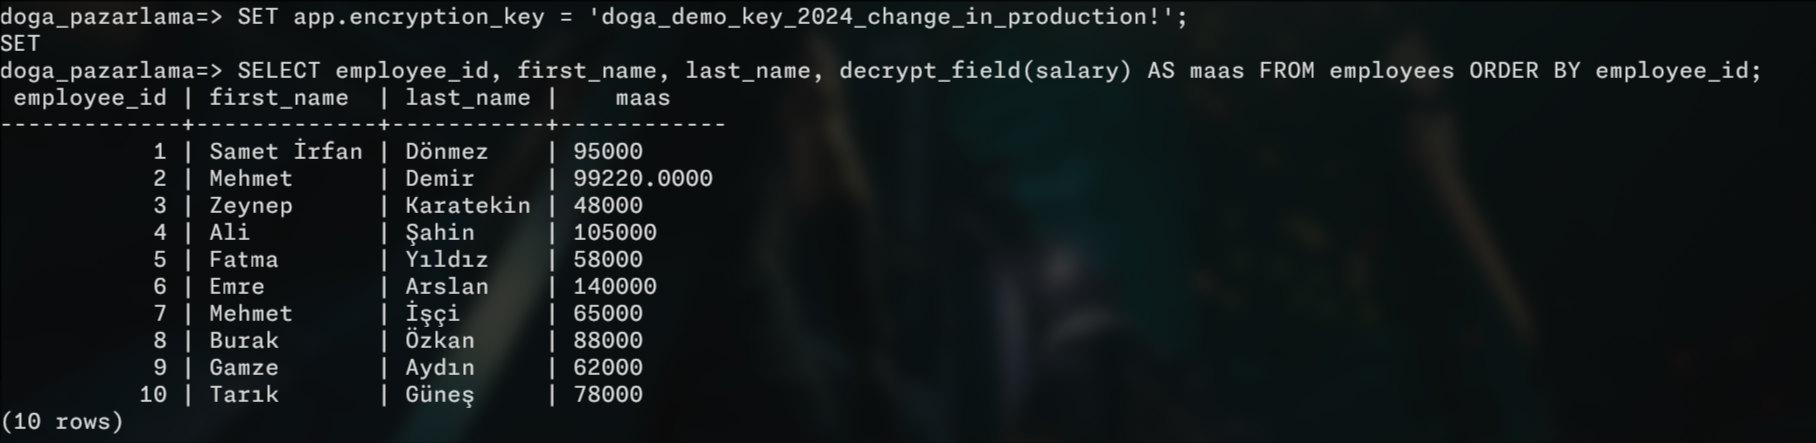
\includegraphics[width=\linewidth]{10_login_decrypt}
  \caption{hr\_manager rolü ile şifreli maaş verisinin çözülmesi}
  \label{fig:login-decrypt}
\end{figure}

\section{Hassas Alanlar İçin Güvenli Görünüm}

\texttt{employees\_public} görünümü maaş sütunu olmaksızın çalışan verilerini sunar. \texttt{readonly\_user}, \texttt{customer\_service} ve \texttt{finance\_analyst} rolleri bu görünüm aracılığıyla çalışan bilgilerine erişebilir; ancak şifreli maaş verisini okuyamazlar:

\begin{lstlisting}[caption={Güvenli görünüm (05\_sifreleme.sql)}]
-- Maas alani olmayan guvenli gorunum
CREATE OR REPLACE VIEW employees_public AS
SELECT employee_id, first_name, last_name, email,
       department, job_title, hire_date
FROM employees;

GRANT SELECT ON employees_public
    TO readonly_user, customer_service, finance_analyst;
\end{lstlisting}

\begin{figure}[h!]
  \centering
  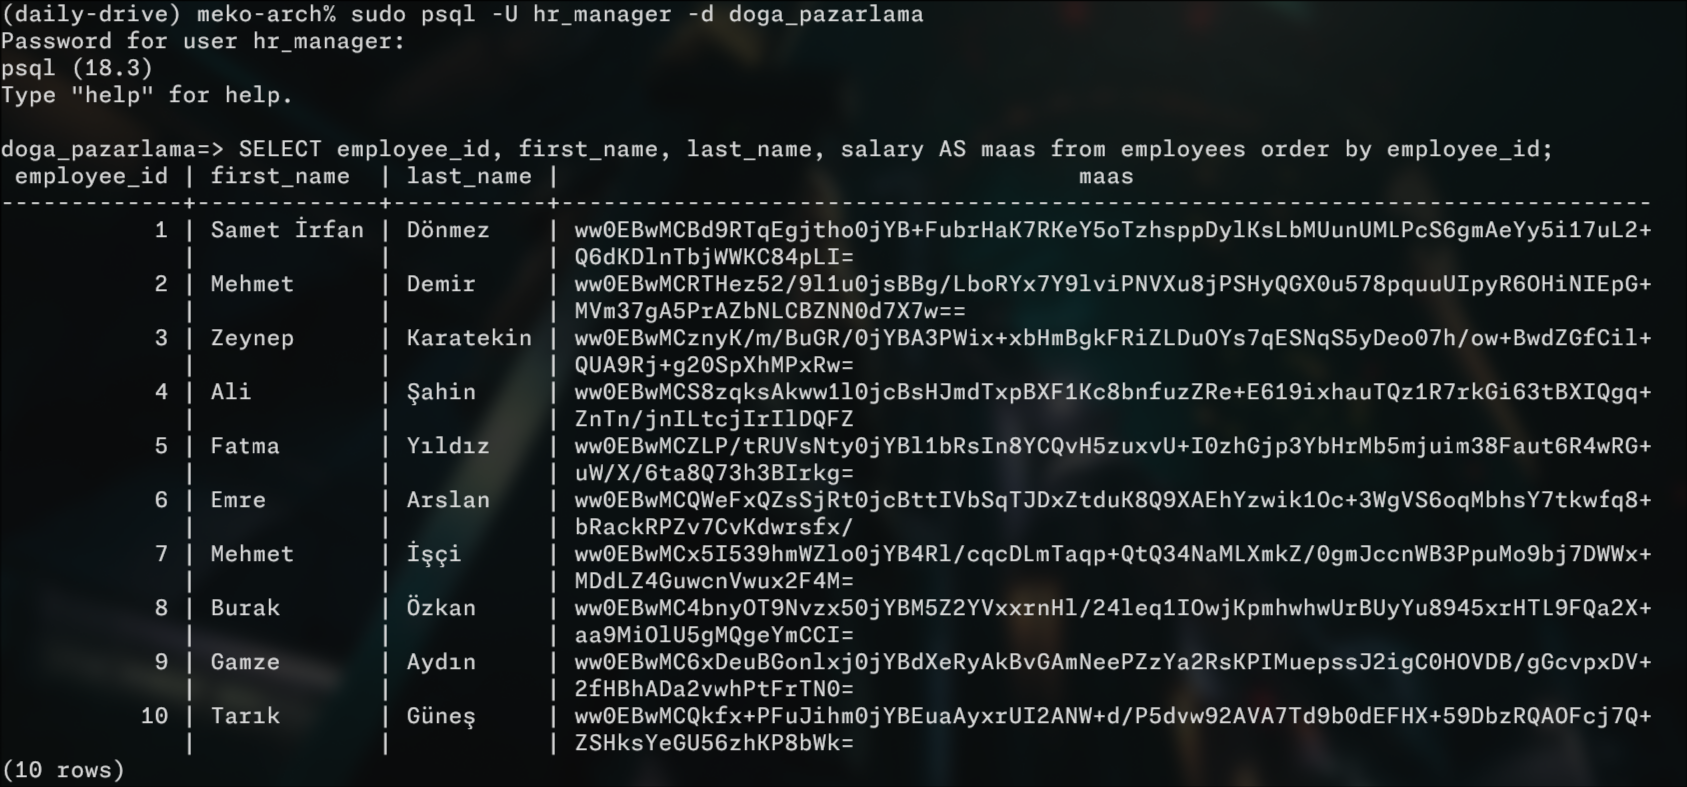
\includegraphics[width=\linewidth]{10_login_and_select}
  \caption{hr\_manager bağlantısı — şifreli maaş sütunu doğrudan sorgulandığında}
  \label{fig:login-select}
\end{figure}

\begin{figure}[h!]
  \centering
  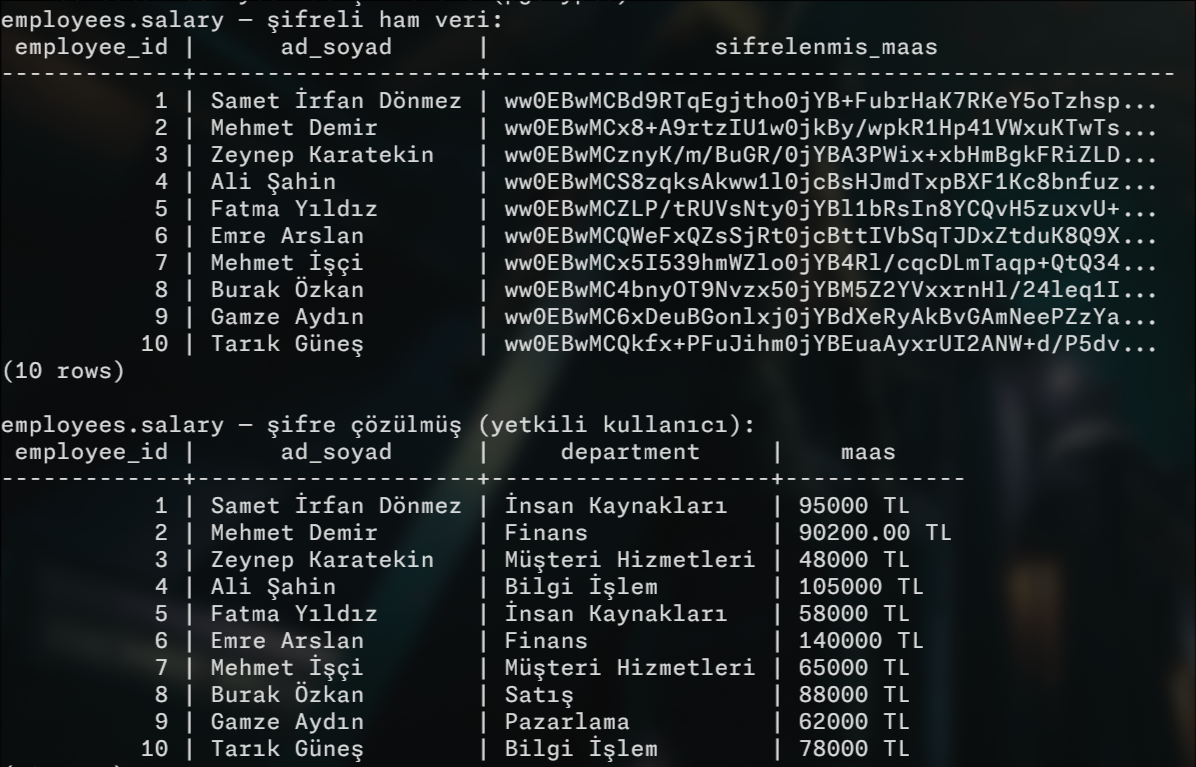
\includegraphics[width=\linewidth]{9_overview_col_level_encryption}
  \caption{Sütun seviyesinde şifreleme — şifreli ve çözülmüş veri karşılaştırması}
  \label{fig:col-enc-overview}
\end{figure}

\begin{block}{Not}
  Gerçek üretim ortamında şifreleme anahtarı veritabanında saklanmamalı; bunun yerine şu seçenekler değerlendirilmelidir:

  \begin{itemize}
    \item \textbf{HashiCorp Vault} — dinamik gizli yönetimi
    \item \textbf{AWS Secrets Manager / Azure Key Vault} — bulut anahtar yönetimi
    \item \textbf{Ortam değişkeni} — konteyner/sistem düzeyinde enjeksiyon
  \end{itemize}
\end{block}

\chapter{SQL Injection Testleri}

\section{SQL Injection Nedir?}

SQL Injection, kullanıcı girdisinin doğrulama yapılmadan SQL sorgusuna eklenmesi sonucu oluşan bir güvenlik açığıdır. Saldırgan özel karakterler (tek tırnak, yorum satırı vb.) kullanarak:
\begin{itemize}
  \item kimlik doğrulamayı atlayabilir,
  \item veritabanındaki gizli verileri okuyabilir,
  \item veri bütünlüğünü bozabilir veya verileri silebilir.
\end{itemize}

\section{Güvensiz Fonksiyon}

\begin{lstlisting}[caption={Güvensiz login fonksiyonu (login\_vulnerable)}]
-- ACIK: kullanici girdisi dinamik SQL'e dogrudan ekleniyor.
v_query := format(
    'SELECT COUNT(*), MAX(role) FROM user_accounts
     WHERE username = ''%s''
       AND password_hash = crypt(''%s'', password_hash)',
    p_username,   -- filtrelenmemis girdi
    p_password    -- filtrelenmemis girdi
);
\end{lstlisting}

\subsection{Saldırı Demosu}

\textbf{Test 1 — Meşru giriş:}
\begin{lstlisting}
SELECT * FROM login_vulnerable('admin', 'Admin@123!');
\end{lstlisting}
\begin{lstlisting}[language={},keywordstyle={},commentstyle={},stringstyle={}]
 basarili |      mesaj      | kullanici_rol
----------+-----------------+---------------
 t        | Giris basarili! | admin
\end{lstlisting}

\textbf{Test 2 — Yanlış şifre:}
\begin{lstlisting}
SELECT * FROM login_vulnerable('admin', 'yanlis_sifre');
\end{lstlisting}
\begin{lstlisting}[language={},keywordstyle={},commentstyle={},stringstyle={}]
 basarili |               mesaj              | kullanici_rol
----------+----------------------------------+---------------
 f        | Hatali kullanici adi veya sifre. |
\end{lstlisting}

\textbf{Test 3 — OR 1=1 injection (username alanı):}
\begin{lstlisting}
SELECT * FROM login_vulnerable(''' OR 1=1 --', 'herhangi_deger');
-- Olusturulan sorgu:
--   WHERE username = '' OR 1=1 --' AND password_hash = ...
--   Tum satirlar eslesiyor; sifre kontrolu yorum satirinda kaldi.
\end{lstlisting}
\begin{lstlisting}[language={},keywordstyle={},commentstyle={},stringstyle={}]
 basarili |      mesaj      | kullanici_rol
----------+-----------------+---------------
 t        | Giris basarili! | user
\end{lstlisting}

\textbf{Test 4 — Yorum satırı injection:}
\begin{lstlisting}
SELECT * FROM login_vulnerable('admin''--', 'herhangi_deger');
-- Olusturulan sorgu:
--   WHERE username = 'admin'--' AND password_hash = ...
--   AND kosulu yorum satirina dustu -> sifre kontrolu yok.
\end{lstlisting}
\begin{lstlisting}[language={},keywordstyle={},commentstyle={},stringstyle={}]
 basarili |      mesaj      | kullanici_rol
----------+-----------------+---------------
 t        | Giris basarili! | admin
\end{lstlisting}

\textbf{Test 5 — UNION injection (kullanıcı adı ve rol sızdırma):}

\texttt{HAVING 1=0} ile orijinal aggregate sonucu bastırılır; yalnızca enjekte edilen satır döner. Böylece \texttt{kullanici\_rol} sütununda tüm \texttt{username:role} çiftleri görünür.

\begin{lstlisting}
SELECT * FROM login_vulnerable(
    ''' HAVING 1=0 UNION SELECT 1,
        string_agg(username || '':'' || role, '', '')
        FROM user_accounts--',
    'x'
);
-- Olusturulan sorgu:
--   SELECT COUNT(*), MAX(role) FROM user_accounts
--   WHERE username = '' HAVING 1=0    -- aggregate satiri yok
--   UNION SELECT 1, string_agg(...)   -- tum kullanicilar dondu
\end{lstlisting}
\begin{lstlisting}[language={},keywordstyle={},commentstyle={},stringstyle={}]
 basarili |      mesaj      | kullanici_rol
----------+-----------------+----------------------------------
 t        | Giris basarili! | admin:admin, app:user, ...
\end{lstlisting}

\begin{figure}[h!]
  \centering
  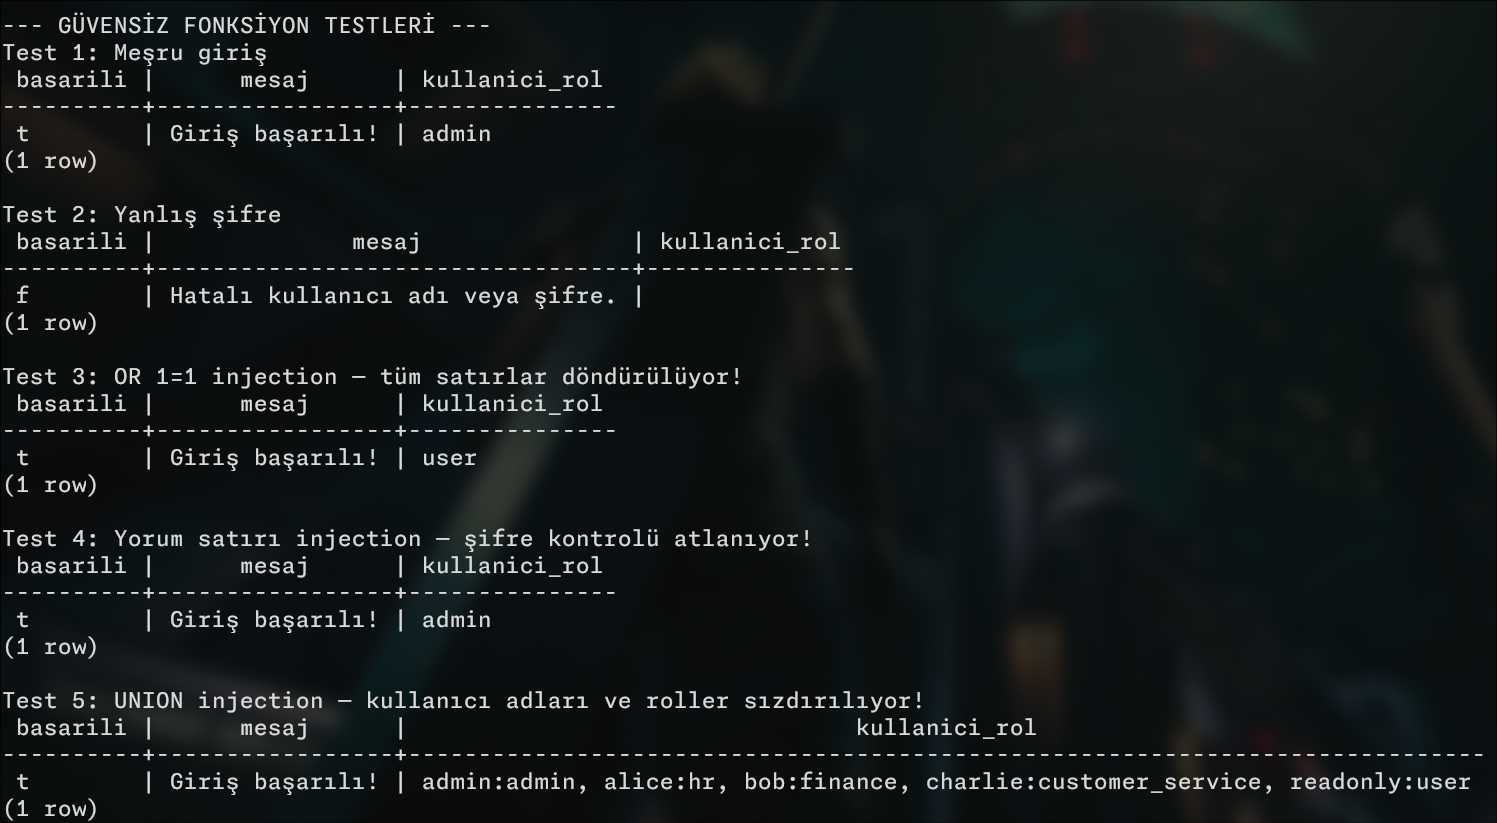
\includegraphics[width=\linewidth]{7_1_sql_injection}
  \caption{Güvensiz fonksiyon test sonuçları — tüm injection saldırıları başarılı}
  \label{fig:sqli-vuln}
\end{figure}

\begin{figure}[h!]
  \centering
  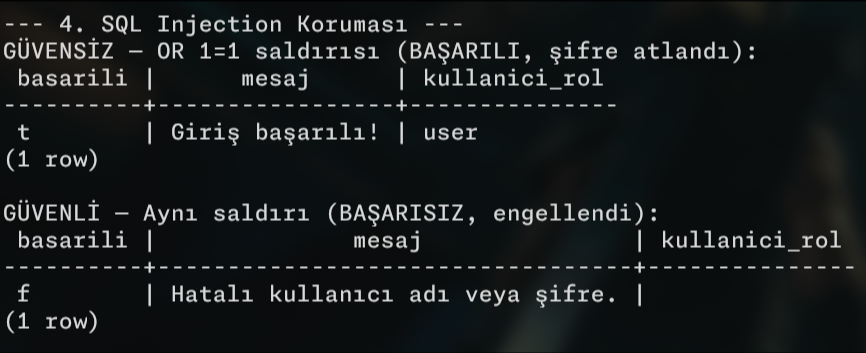
\includegraphics[width=\linewidth]{9_overview_sql_injection}
  \caption{OR 1=1 saldırısı — güvensiz vs güvenli fonksiyon karşılaştırması (08\_demo.sql)}
  \label{fig:sqli-overview}
\end{figure}

\section{Güvenli Fonksiyon}

Çözüm: parametreli sorgular (Prepared Statement). Kullanıcı girdisi SQL kodu olarak değil, \textbf{veri} olarak işlenir.

\begin{lstlisting}[caption={Güvenli login fonksiyonu (login\_safe)}]
-- GUVENLI: parametre baglama; p_username SQL kodu olarak yorumlanamaz.
SELECT password_hash, role
INTO   v_stored_hash, v_role
FROM   user_accounts
WHERE  username = p_username;

-- Bcrypt karsilastirmasi
v_success := (
    v_stored_hash IS NOT NULL
    AND crypt(p_password, v_stored_hash) = v_stored_hash
);

-- Saldiri payload'lari cok uzun olabileceginden 50 karaktere kirpilir.
INSERT INTO login_attempts (username, ip_address, success)
VALUES (LEFT(p_username, 50), p_ip_address, v_success);
\end{lstlisting}

Güvenli fonksiyona aynı payload uygulandığında:
\begin{itemize}
  \item \texttt{' OR 1=1 -{}-} → \texttt{username} alanında literal string olarak aranır; bulunamaz, giriş başarısız.
  \item \texttt{admin'-{}-} → veritabanında bu kullanıcı adı mevcut değil; giriş başarısız.
  \item UNION payload → kullanıcı adı olarak aranır; bulunamaz, giriş başarısız; veri sızıntısı önlenir.
\end{itemize}

\begin{figure}[h!]
  \centering
  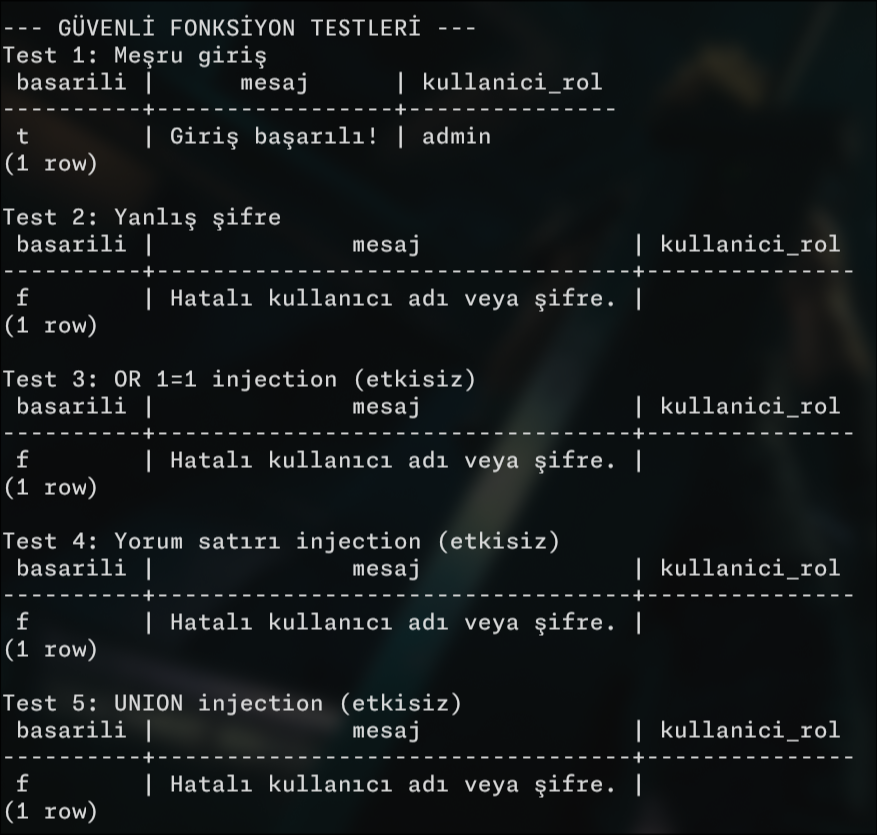
\includegraphics[width=\linewidth]{7_2_sql_injection}
  \caption{Güvenli fonksiyon test sonuçları — tüm saldırılar etkisiz}
  \label{fig:sqli-safe}
\end{figure}

\begin{figure}[h!]
  \centering
  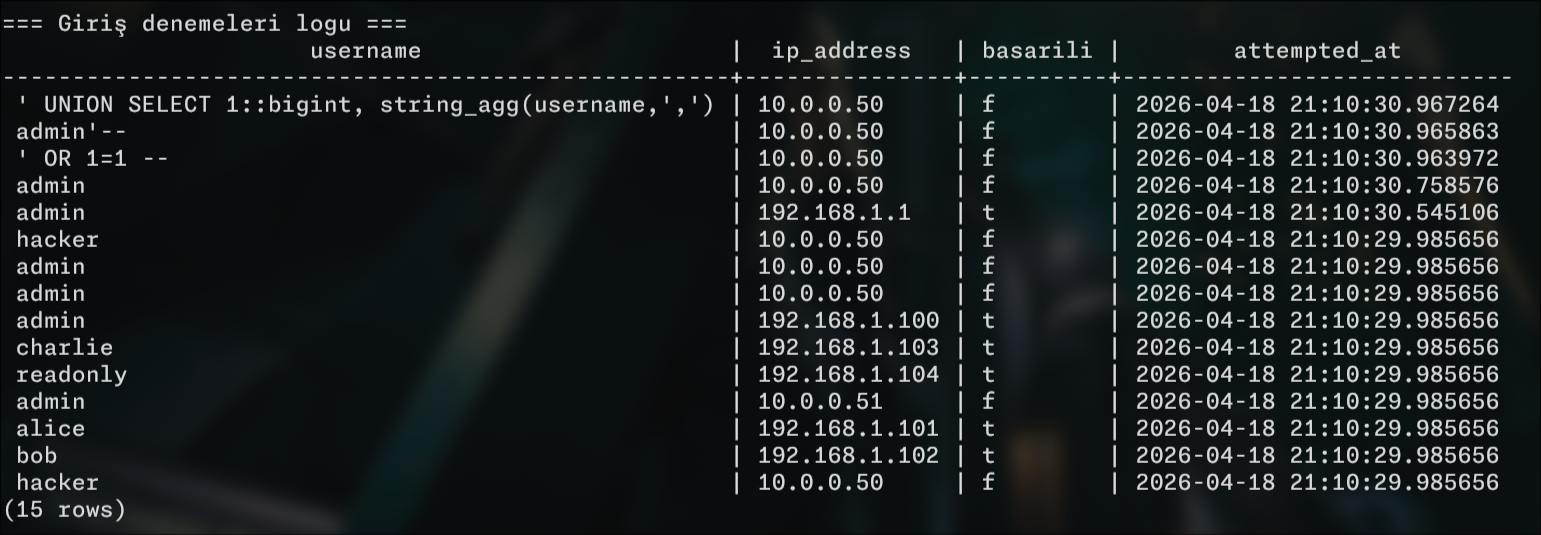
\includegraphics[width=\linewidth]{7_3_sql_injection_logs}
  \caption{Giriş denemeleri logu — injection payload'ları kayıt altında}
  \label{fig:sqli-logs}
\end{figure}

\begin{figure}[h!]
  \centering
  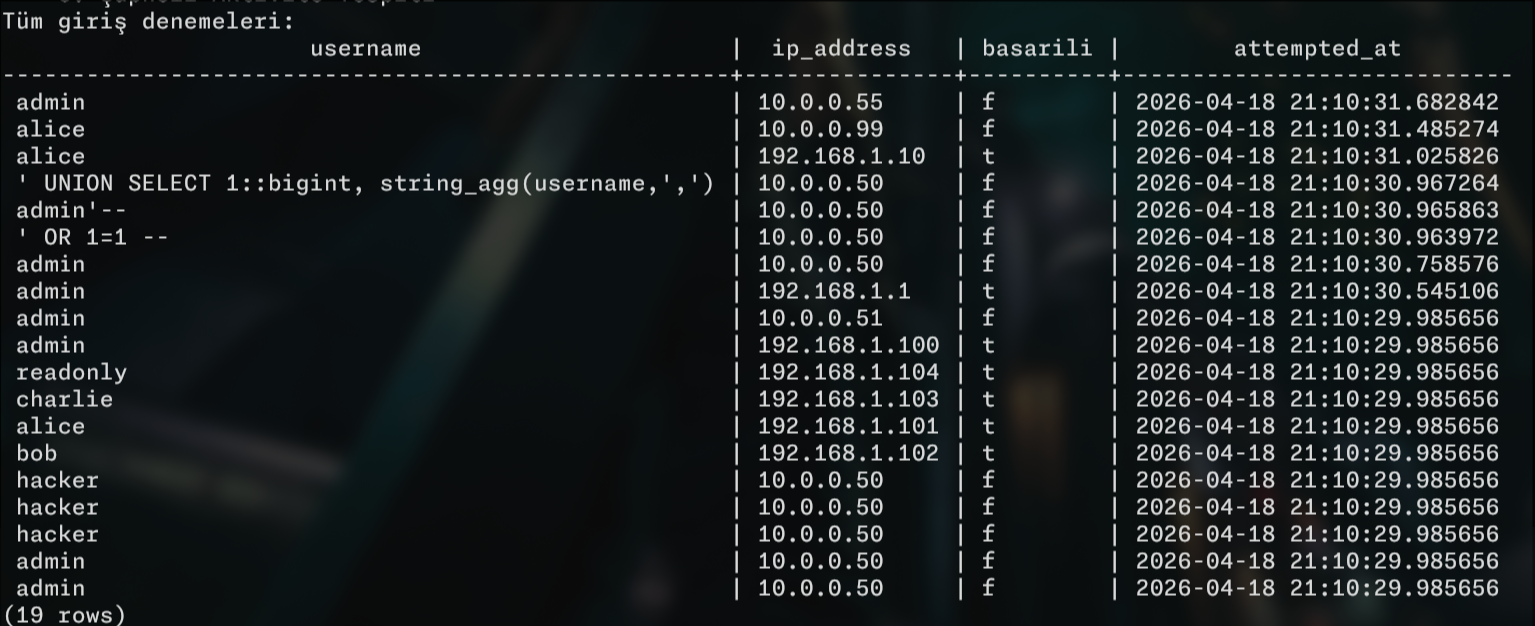
\includegraphics[width=\linewidth]{9_overview_login_attempts}
  \caption{Tüm giriş denemeleri — başarılı ve başarısız denemeler (08\_demo.sql)}
  \label{fig:login-attempts-overview}
\end{figure}

\section{Uygulama Seviyesi Şifreli Kimlik Doğrulama}

\texttt{user\_accounts} tablosunda şifreler \textbf{bcrypt} ile hash'lenerek saklanmaktadır:

\begin{lstlisting}[caption={bcrypt ile şifre hash'leme (02\_ornek\_veri\_ekle.sql)}]
INSERT INTO user_accounts (username, email, password_hash, role) VALUES
('admin', 'admin@doga.com',
 crypt('Admin@123!', gen_salt('bf', 12)),  -- maliyet faktoru: 12
 'admin');
\end{lstlisting}

\begin{figure}[h!]
  \centering
  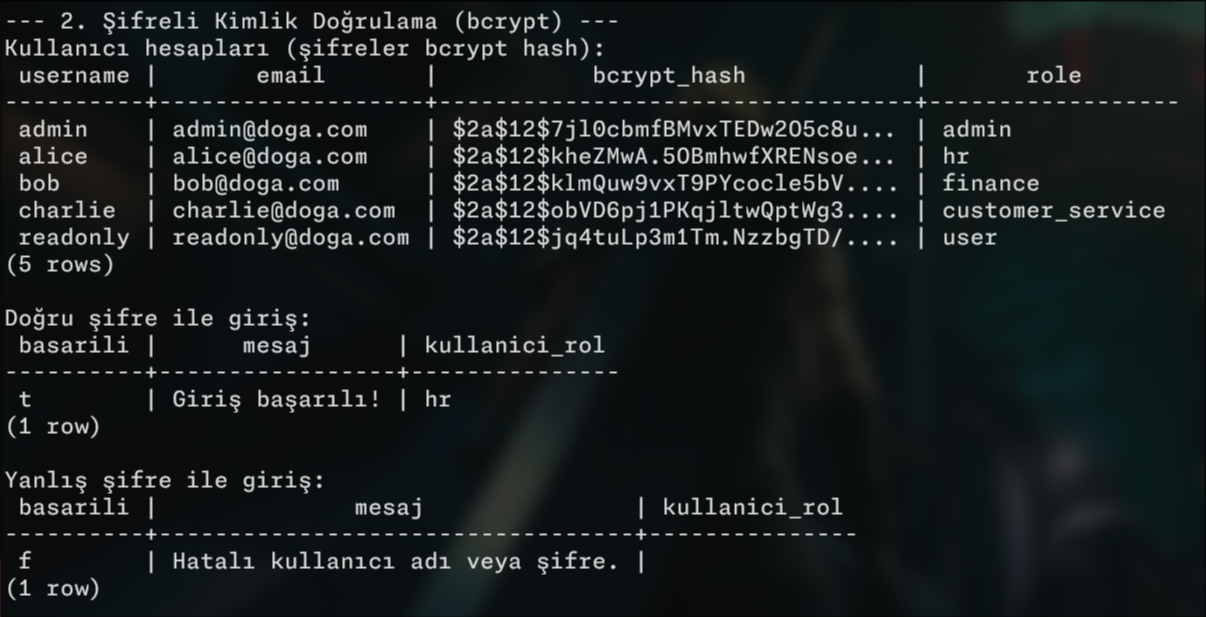
\includegraphics[width=\linewidth]{9_overview_encrypted_login}
  \caption{Kullanıcı hesapları — bcrypt hash'lenmiş şifreler ve doğrulama testi}
  \label{fig:bcrypt-overview}
\end{figure}

\texttt{gen\_salt('bf', 12)} Blowfish algoritmasını maliyet faktörü 12 ile kullanır; bu değer arttıkça hash hesaplama yavaşlar ve kaba kuvvet (brute-force) saldırıları zorlaşır.

% =============================================================
\chapter{Denetim Günlükleri}
% =============================================================

\section{Tetikleyici Tabanlı Audit Logging}

Her hassas tablodaki (\texttt{employees}, \texttt{customers}, \texttt{transactions}, \texttt{user\_accounts}) \texttt{INSERT}/\texttt{UPDATE}/\texttt{DELETE} işlemi otomatik olarak \texttt{audit\_log} tablosuna kaydedilir.

\begin{lstlisting}[caption={Denetim günlüğü tablosu}]
CREATE TABLE IF NOT EXISTS audit_log (
    log_id      SERIAL       PRIMARY KEY,
    table_name  VARCHAR(50)  NOT NULL,
    operation   VARCHAR(10)  NOT NULL
                             CHECK (operation IN ('INSERT','UPDATE','DELETE')),
    old_data    JSONB,     -- UPDATE/DELETE oncesi durum
    new_data    JSONB,     -- INSERT/UPDATE sonrasi durum
    changed_by  VARCHAR(100) NOT NULL DEFAULT current_user,
    changed_at  TIMESTAMP    NOT NULL DEFAULT NOW()
);
\end{lstlisting}

\section{Tetikleyici Fonksiyonu}

\begin{lstlisting}[caption={Genel amaçlı audit trigger (07\_audit\_log.sql)}]
CREATE OR REPLACE FUNCTION audit_trigger_func()
RETURNS TRIGGER LANGUAGE plpgsql SECURITY DEFINER AS $$
BEGIN
    INSERT INTO audit_log (table_name, operation, old_data, new_data, changed_by)
    VALUES (
        TG_TABLE_NAME,
        TG_OP,
        CASE WHEN TG_OP = 'INSERT' THEN NULL ELSE to_jsonb(OLD) END,
        CASE WHEN TG_OP = 'DELETE' THEN NULL ELSE to_jsonb(NEW) END,
        current_user
    );
    RETURN CASE WHEN TG_OP = 'DELETE' THEN OLD ELSE NEW END;
END; $$;

-- Tetikleyiciyi tum hassas tablolara uygula
CREATE TRIGGER employees_audit
    AFTER INSERT OR UPDATE OR DELETE ON employees
    FOR EACH ROW EXECUTE FUNCTION audit_trigger_func();

CREATE TRIGGER customers_audit
    AFTER INSERT OR UPDATE OR DELETE ON customers
    FOR EACH ROW EXECUTE FUNCTION audit_trigger_func();

CREATE TRIGGER transactions_audit
    AFTER INSERT OR UPDATE OR DELETE ON transactions
    FOR EACH ROW EXECUTE FUNCTION audit_trigger_func();

CREATE TRIGGER user_accounts_audit
    AFTER INSERT OR UPDATE OR DELETE ON user_accounts
    FOR EACH ROW EXECUTE FUNCTION audit_trigger_func();
\end{lstlisting}

\texttt{SECURITY DEFINER} sayesinde trigger fonksiyonu, fonksiyonu tanımlayan kullanıcının yetkileriyle çalışır. Bu sayede \texttt{audit\_log} tablosuna diğer roller INSERT yapamamasına rağmen tetikleyici aracılığıyla kayıt düşebilir.

\section{Şüpheli Aktivite Tespiti}

\texttt{suspicious\_login\_activity} fonksiyonu belirli bir süre içinde eşik değerini aşan başarısız giriş denemelerini raporlar:

\begin{lstlisting}[caption={Şüpheli aktivite fonksiyonu}]
-- Son 30 dakikada ucten fazla basarisiz deneme yapan kullanici ve IP ikilileri
SELECT * FROM suspicious_login_activity(30, 3);
\end{lstlisting}

\begin{figure}[h!]
  \centering
  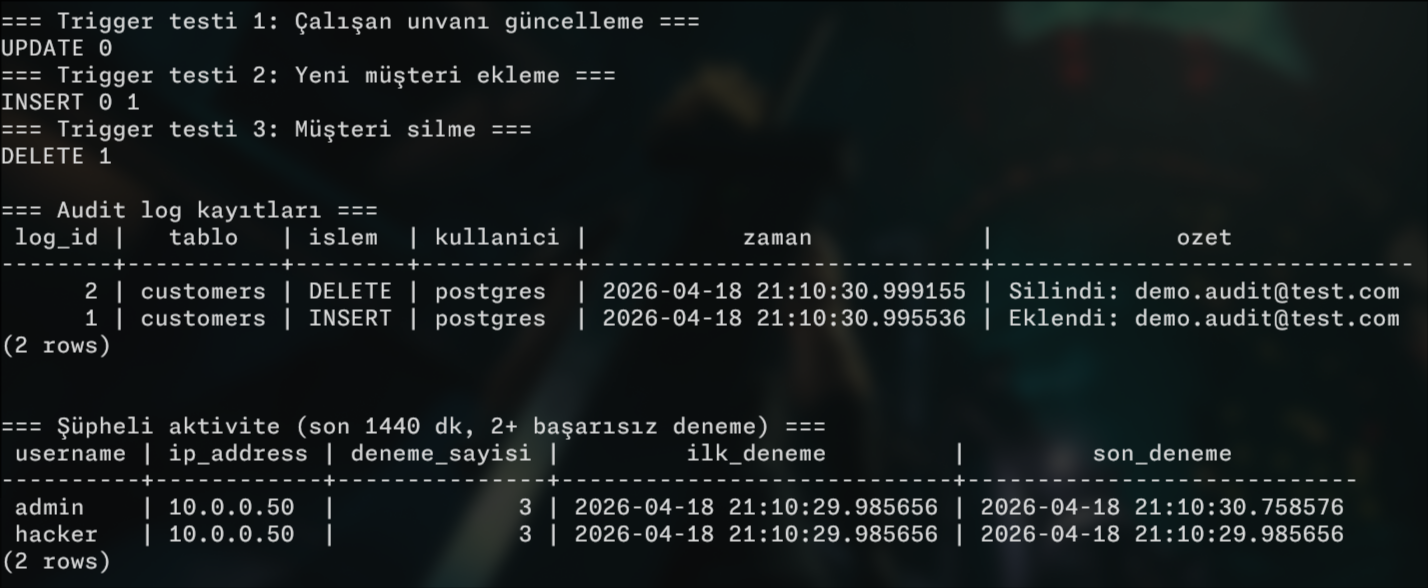
\includegraphics[width=\linewidth]{8_audit_log}
  \caption{Denetim günlüğü — tetikleyici tabanlı değişiklik kaydı ve şüpheli aktivite tespiti}
  \label{fig:audit-log}
\end{figure}

\begin{figure}[h!]
  \centering
  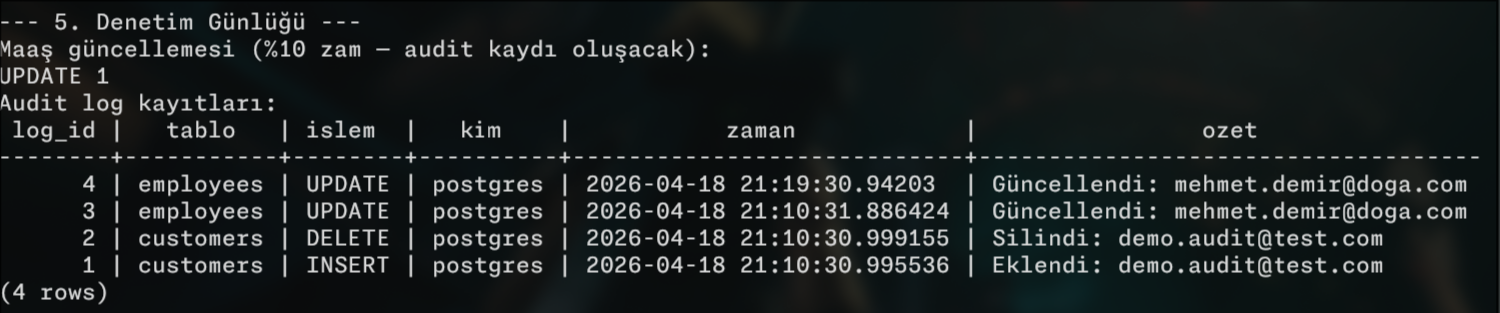
\includegraphics[width=\linewidth]{9_overview_audit_log}
  \caption{Denetim günlüğü genel bakış — UPDATE ve DELETE kayıtları (08\_demo.sql)}
  \label{fig:audit-overview}
\end{figure}

Örnek çıktı (seed verileri): \texttt{10.0.0.50} IP adresi \texttt{admin} ve \texttt{hacker} kullanıcıları için birden fazla başarısız deneme yapmıştır.

% =============================================================
\chapter{Sonuç}
% =============================================================

Bu projede PostgreSQL üzerinde çok katmanlı bir veritabanı güvenlik altyapısı tasarlanıp uygulanmıştır:

\begin{itemize}
  \item \textbf{Kimlik Doğrulama}: Tüm roller \texttt{scram-sha-256} protokolüyle korunan şifrelere sahiptir. \texttt{pg\_hba.conf} yapılandırmasıyla hem yerel hem ağ bağlantıları için şifreli doğrulama zorunlu kılınmıştır.
  \item \textbf{Yetkilendirme}: En az ayrıcalık ilkesiyle her rol yalnızca iş işlevine uygun tablolara erişebilir. RLS ile çalışan verilerine satır düzeyinde filtreleme uygulanmıştır.
  \item \textbf{Veri Gizliliği}: Maaş, kredi kartı ve kimlik numarası gibi hassas alanlar \texttt{pgcrypto} ile şifreli tutulmaktadır. Şifre çözme yetkisi yalnızca ihtiyaç duyan rollere verilmiştir.
  \item \textbf{Uygulama Güvenliği}: Güvenli giriş fonksiyonu parametreli sorgular kullanarak SQL injection saldırılarını engeller; her giriş denemesi izlenmektedir.
  \item \textbf{İzlenebilirlik}: Tetikleyici tabanlı denetim sistemi tüm veri değişikliklerini JSONB formatında kayıt altına alır; şüpheli aktivite tespiti için analiz fonksiyonu hazırlanmıştır.
\end{itemize}

Bu katmanların birlikte çalışması, \textit{savunma derinliği (defense in depth)} prensibine uygun bir güvenlik modeli ortaya koymaktadır: bir katmanın aşılması durumunda diğer katmanlar korumaya devam eder.

\end{document}
